\newpage{\thispagestyle{empty}\cleardoublepage}
\chapter{dyngen: simulating single cells} 
\chaptermark{dyngen: simulating single cells}
\label{chap:dyngen}

\begin{quote}
	\textbf{Abstract:} 
\end{quote}

\vfill

Adapted from:\\

\newpage

\section{Introduction}
Continuous technological advancements to high-throughput profiling of single cells
are having profound effects on how researchers can validate biological hypotheses. 
For example, single-cell RNA sequencing (scRNA-seq) directly resulted in the development
of a new type of computational method called trajectory inference (TI). By profiling
the transcriptomics profiles of developing cells, TI methods attempt to reconstruct 
and characterise the underlying dynamic processes \cite{cannoodt_computationalmethodstrajectory_2016}.
While early experimental technologies allowed to profile one single modality (e.g. DNA sequence, 
RNA or protein expression), recent developments permit profiling multiple modalities simultaneously.

An ideal experiment would be able to observe all aspects of a cell, including a full history of its 
molecular states, spatial positions and environmental interactions \cite{stuart_integrativesinglecellanalysis_2019}. 
While this falls outside the reach of current experimental technologies, \textit{in silico} simulations
of single cells would allow developing the next wave of computational techniques
in anticipation of new experimental technologies.

A few generators of scRNA-seq profiles have already been developed (e.g. splatter \cite{zappia_splattersimulationsinglecell_2017} and PROSSTT \cite{papadopoulos_prossttprobabilisticsimulation_2018}). These can be 
used to evaluate the performance of computational tools, and to explore their strengths and weaknesses. A limitation of directly simulating a scRNA-seq profile (instead of a single cell) is that extending the simulation to other aspects of the cell -- such as tracking the full history of molecular states -- becomes difficult.

We introduce dyngen, a multi-modality simulator of single cells (Figure \ref{fig:dyngen}).
dyngen was initially developed as part of a comprehensive benchmark of TI methods \cite{saelens_comparisonsinglecelltrajectory_2019} but has since been extended to be applicable in a much broader context.
We demonstrate its flexibility by simulating numerous different types of biological experiments, and using these simulations to develop new benchmarking techniques for computational tools.

\begin{figure}
	\centering
	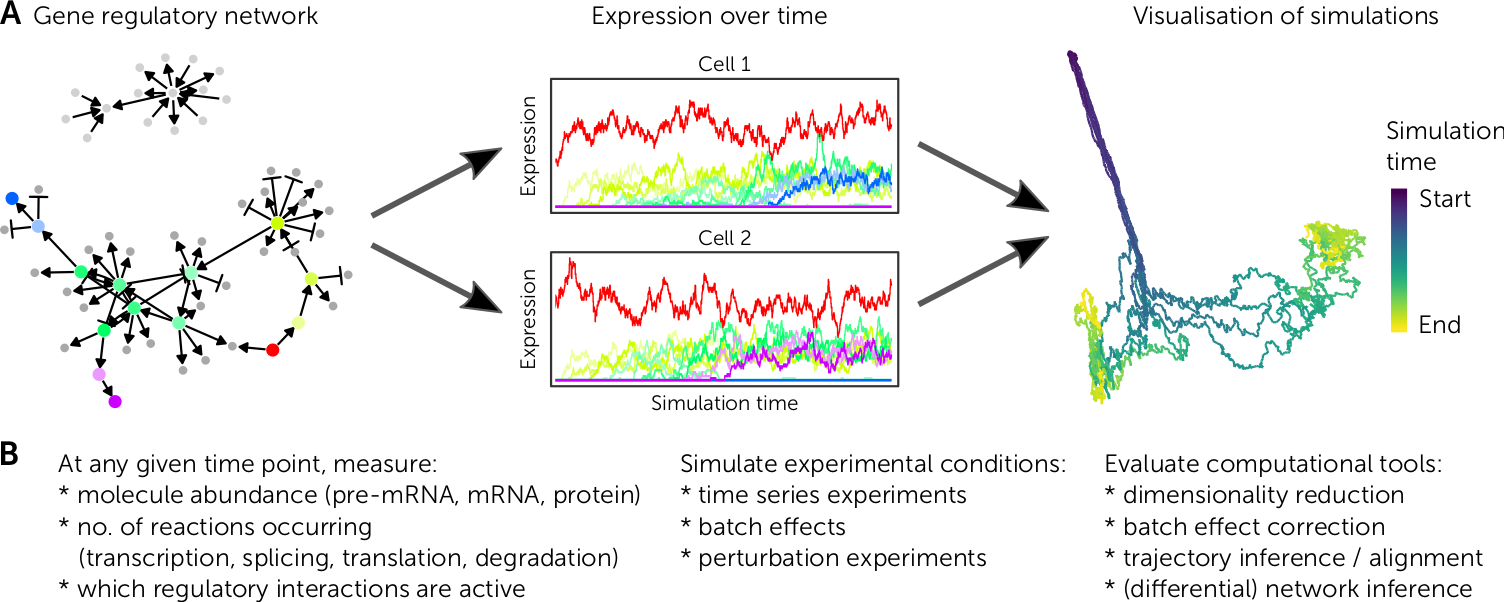
\includegraphics[width=\linewidth]{fig/dyngen/showcase_3.png} 
	\caption{Showcase of dyngen functionality. \textbf{TODO: change to pdf.} Remove B?} % TODO: update label
	\label{fig:dyngen}
\end{figure}

\section{Results}
dyngen is a simulator for single cells that develop over time. Throughout this section, a simple simulation of a cell undergoing a cyclic process is used to illustrate key strengths of dyngen (Figure \ref{fig:simplecyclic}). This example only comprises of a single cell containing 5 genes, but dyngen can easily scale up to thousands of simulations containing thousands of genes.

In dyngen, a cell consists of a set of molecules, the abundance of which are affected by a set of reactions: transcription, splicing, translation, and degradation (Figure \ref{fig:simplecyclic}A). These reactions are determined from a predefined set of gene regulatory interactions (Figure \ref{fig:simplecyclic}B), henceforth referred to as a gene regulatory network (GRN). The likelihood of a reaction occurring at any given point in time is defined by the GRN and by the abundance of molecules involved each reaction.

One of dyngen's main advantages is that through careful engineering of the GRN, different cellular developmental processes can be obtained. Different GRNs can result in branching, converging, cyclic, or even disconnected developmental topologies. Multiple simulations with slightly different GRNs can emulate rewiring events in disease or perturbation experiments. % could use figure; one with GRNs of different topologies, another with rewiring events
Multiple simulations with different initial molecule abundance levels can be used to replicate batch effects. 

\begin{figure}
	\centering
	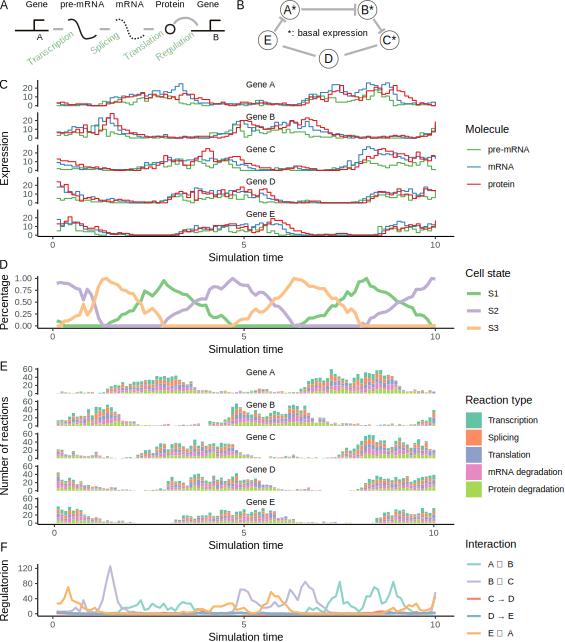
\includegraphics[width=\linewidth]{fig/dyngen/simplecyclic_edited} 
	\caption{Showcase of dyngen functionality.}
	\label{fig:simplecyclic}
\end{figure}

Another advantage is that dyngen returns many modalities throughout the whole simulation: molecular abundance (Figure \ref{fig:simplecyclic}C), cellular state (\ref{fig:simplecyclic}D), number of reaction firings (\ref{fig:simplecyclic}E), reaction likelihoods (not shown), and regulation activations (\ref{fig:simplecyclic}F). These modalities can serve as input data and ground truth for benchmarking many types of computational approaches, including clustering, batch effect correction, dimensionality reduction, trajectory inference, trajectory alignment, and gene regulatory network inference. 

The final main advantage is that by making alterations to the generation pipeline, multiple types of experiments can be simulated. The default settings assumes an asynchronous dynamic process and thus cells are sampled uniformly. A time-series experiment of a synchonised dynamic process can be simulated by sampling cells from various intervals of the simulation. 
% TODO: you can even profile the same cell at regular intervals, which is a technology that does not exist yet at a single cell omics scale. This could be used to evaluate, for example, RNA velocity approaches.

%\subsection{Example simulation}
%
%
%\begin{figure}
%	\centering
%	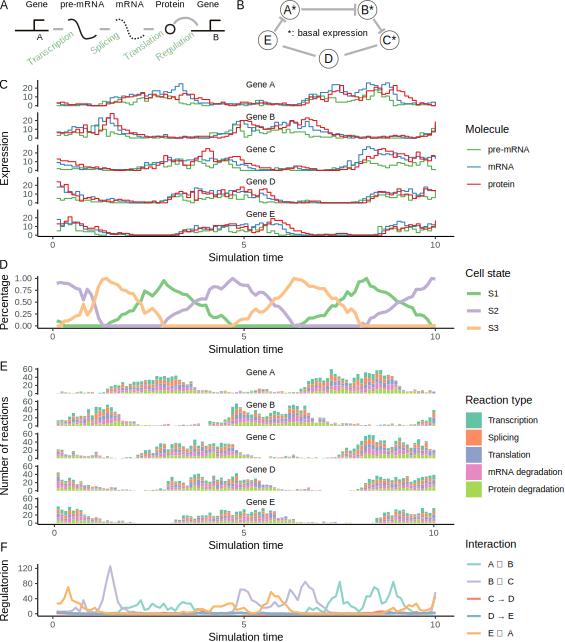
\includegraphics[width=\linewidth]{fig/dyngen/simplecyclic_edited} 
%	\caption{Simple cyclic} % TODO: update label
%	\label{fig:simplecyclic}
%\end{figure}

\subsection{Applications}

\subsection{Supported backbones}

\subsection{Backbone lego}

\subsection{Additional experimental effects}
% time series, batch effects, perturbation experiments


\section{Discussion}
% cell cycle, mitosis
% cell-cell interaction
% spatial + cell movement
% transcriptional bursting
% add mechanism for triggering reactions only when they are needed?

\section{Methods}

\subsection{Simulating a snapshot experiment with dyngen}
\subsubsection{Define the module network and the state network}
\subsubsection{Generate the transcription factor network}
\subsubsection{Generate targets and housekeeping genes}
\subsubsection{Convert gene regulatory network to a set of SSA reactions}
\subsubsection{Determine the gold standard}
\subsubsection{Running SSA simulations and mapping it to the gold standard}
\subsubsection{Simulate snapshot experiment}
\subsection{Predefined backbones}

\subsection{Other types of experiments}
\subsubsection{Time series experiment}
\subsubsection{Perturbation experiment}
\subsubsection{Batch effects}
\subsection{Evaluating computational tools}
\subsubsection{Clustering}
\subsubsection{Dimensionality reduction}
\subsubsection{Batch effect correction}
\subsubsection{Trajectory inference}
\subsubsection{Trajectory alignment}
\subsubsection{Network inference}







%dyntoy and PROSSTT are specifically developed to generate datasets
% containing single cells which develop along a certain trajectory.
% These generators start a certain topology in mind, 
% simulate changing gene expressions along each of the branches of the topology, and sample cells
% from random points in the trajectory. splatter is focused on well replicating the specific noise characteristics of
% scRNA-seq data, and simulates differentially expressed genes in order to replicate clusters of cells, batch effects
% and even trajectories. dyngen 1.0 borrows a page from GeneNetWeaver in that it also converts a GRN into an ODE, but
% the GRN is constructed in such a way that the repeated simulations resemble single cells following a regulatory program
% (e.g. differentiation into one of two celltypes). BoolODE uses the dyngen 1.0 GRNs but uses boolean models to convert 
% the network into an ODE, and is used to evaluate the performance of NI methods, not TI methods. 

%\begin{table}
%	\caption{\textbf{Comparison of existing single-cell omics simulators.} TI: trajectory inference, NI: network inference, Cl: clustering, DR: dimensionality reduction.} \label{tab:simulators}
%	\centering\fontsize{9}{11}\selectfont
%	\begin{tabularx}{\linewidth}{p{1.6cm}p{2.5cm}p{3cm}X}
%		Generator & Used to evaluate & Data type(s) & Approach \\ \hline
%		dyngen 1.0 & TI & mRNA \& protein & GRN, ODE, Euler--Maramuya \\
%		dyntoy & TI & mRNA & Visualise tree in plane, generate expression in plane, sample cells from tree \\
%		PROSSTT & TI & mRNA & Random walks along tree, sample cells from tree \\
%		splatter & Cl \& TI & mRNA & Simulate DE genes, simulate scRNA-seq noise \\
%		BoolODE & NI & mRNA \& protein & Use dyngen GRN's, ODE, Euler--Maramuya \\
%		dyngen 2.0 & TI, NI, Cl, DR & pre-mRNA, mRNA, protein & Backbone, GRN, SSA \\
%		dyngen 3? & TI, NI, Cl, DR & pre-mRNA, mRNA, miRNA, protein, protein complex & Backbone, GRN, SSA
%	\end{tabularx}
%\end{table}